\newpage		
	\section*{Лист 1}
		
		\subsection*{1}
		\subsubsection*{\textbf{А}}
		Рассмотрим треугольник в модели Пуанкаре, его вершины соответствуют каким-то трем точкам $\frac{p_1}{q_1}, \frac{p_2}{q_2}, \frac{p_3}{q_3}$. Запишем условия касания орициклов с этими координатами, выведя их из теоремы Пифагора:
		\begin{gather*}
			\Big(\frac{p_1}{q_1} - \frac{p_2}{q_2}\Big)^2 = 
			\Big(\frac{1}{2q_1^2} + \frac{1}{2q_2^2}\Big)^2 - \Big(\frac{1}{2q_1^2} - \frac{1}{2q_2^2}\Big)^2 = 
			\frac{1}{q_1^2 q_2^2}\\
			\Big(\frac{p_1}{q_1} - \frac{p_3}{q_3}\Big)^2 = 
			\Big(\frac{1}{2q_1^2} + \frac{1}{2q_3^2}\Big)^2 - \Big(\frac{1}{2q_1^2} - \frac{1}{2q_3^2}\Big)^2 = 
			\frac{1}{q_1^2 q_3^2}\\
			\Big(\frac{p_3}{q_3} - \frac{p_2}{q_2}\Big)^2 = 
			\Big(\frac{1}{2q_3^2} + \frac{1}{2q_2^2}\Big)^2 - \Big(\frac{1}{2q_3^2} - \frac{1}{2q_2^2}\Big)^2 = 
			\frac{1}{q_3^2 q_2^2}
		\end{gather*}
		Тогда остается заметить, что $\frac{p_1}{q_1}, \frac{p_2}{q_2}, \frac{p_3}{q_3}$ нам известны, так как нам извесны вершины треугольников, а следовательно из данной системы уравнений мы получим $q_1, q_2, q_3$ (так как в левой части каждого из уравнений находится некое число, а в правой произведение неизвестных), а следовательно и $p_1, p_2, p_3$ (домножив $\frac{p_1}{q_1}, \frac{p_2}{q_2}, \frac{p_3}{q_3}$ на $q_1, q_2, q_3$). И тогда мы однозначно зададим орициклы, тем самым доказав что такая тройка единственная.
		
		
		
		\subsubsection*{\textbf{Б}}
		Докажем от противного, тогда точка касания орициклов не всегда расположена на стороне треугольника.\\
		\begin{figure}[h]
			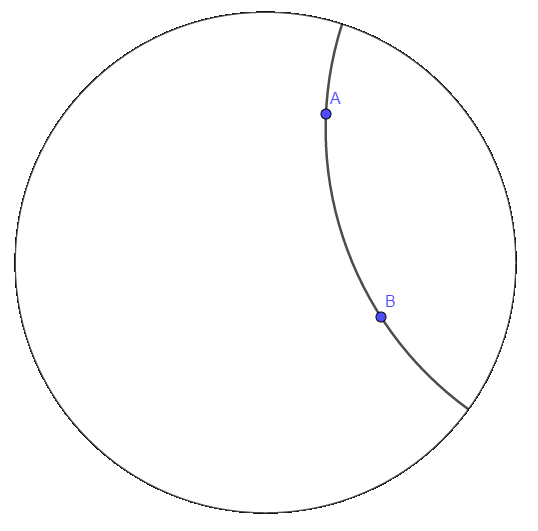
\includegraphics[width=0.5\linewidth]{pic7}
		\end{figure}\\
		\noindent
		Рассмотрим тот случай когда она вне стороны, тогда она пересекает орициклы в каких-то точках, причем в этих точках она также перпендикулярная орициклам(это следует из свойств орицикла и из того, что данная геодезическая заканчивается в основании орицикла). Тогда рассмотрим треугольник образованный точками пересечения геодезической с орициклами и точкой касания орициклов, углы при пересечении геодезической равны $90^{\circ}$, а следовательно сумма углов данного треугольника хотя бы $180^{\circ}$, чего быть не может так как сумма углов треугольника в данной плоскости менее $180^{\circ}$, противоречие. \\
		Следовательно геодезическая с концами в основаниях касающихся орициклах обязана проходить через их точку касания.
		
		
		
		\subsection*{2}
		\subsubsection*{\textbf{А}}
		Для удобства бозначим орицикл как $O = o(p,q) = \frac{p}{q}$, геодезическую как $g$, расстояние между ними как $d(O, g) = d(o(p,q), g)$.\\
		Тогда рассмотрим\\
		\begin{figure}[h]
			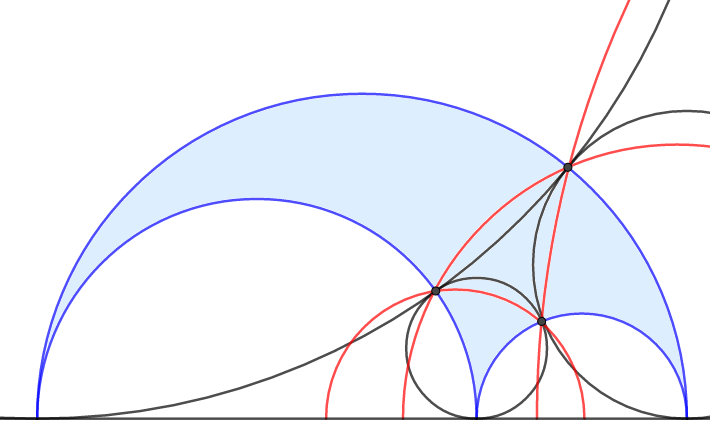
\includegraphics[width=0.5\linewidth]{pic1}\\
			\text{Синим отмечен треугольник, красным отмечены средние линии}
		\end{figure}\\
		\noindent
		Заметим, что мы можем провести проективное преобразование, так как проективное преобразование -- это дробно-линейное преобразование вида $x \to \frac{ax+b}{cx+d}$, что и есть преобразование в модели верхней полуплоскости Пуанкаре при $ac-bd>0$. Пусть наше преобразование переводит точки $\frac{p_1}{q_1}, \frac{p_2}{q_2}, \frac{p_3}{q_3}$ в точки $0, 1, \infty$, тогда мы получим картинку:\\
		\begin{figure}[h]
			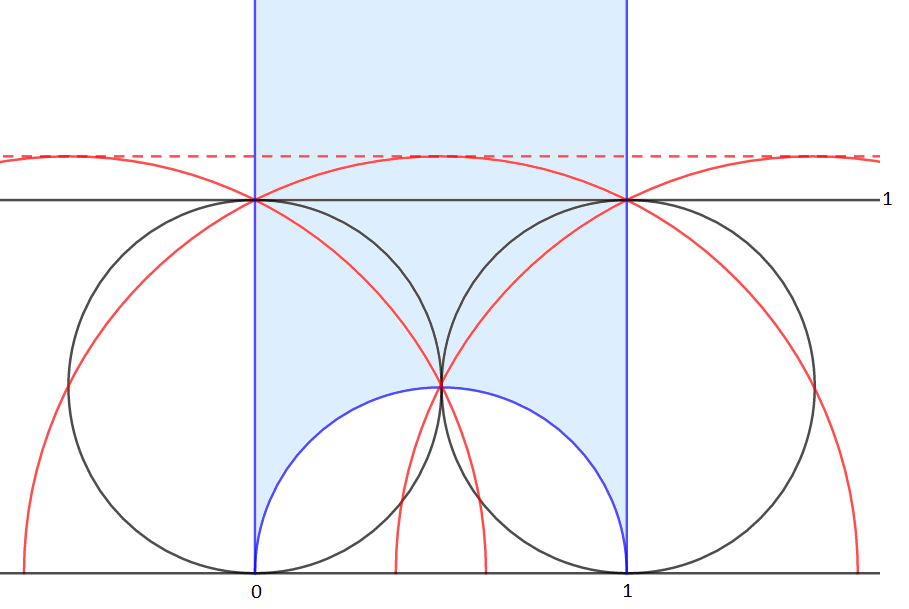
\includegraphics[width=0.5\linewidth]{pic2}
		\end{figure}\\
		\noindent
		Заметим, что орицикл $O_{A_1}$ в точке $0$ теперь имеет вид $\frac{0}{1}$, $O_{A_2}$ в точке $1$ имеет вид $\frac{1}{1}$, $O_{A_3}$ в $\infty$ имеет вид $\frac{1}{0}$.\\ Тогда рассмотрим расстояния от этих орициклов до средних линий. Заметим что в этом случае средние линии имеют координаты концов: $\{\frac{1}{2}-\frac{\sqrt{5}}{2}, \frac{1}{2}+\frac{\sqrt{5}}{2}\},\ \{-\frac{1}{2}-\frac{\sqrt{5}}{2}, -\frac{1}{2}+\frac{\sqrt{5}}{2}\},\ \{\frac{3}{2}-\frac{\sqrt{5}}{2}, \frac{3}{2}+\frac{\sqrt{5}}{2}\}$\\
		Рассотрим линию, пересекающую две вертикальных стороны треугольника. Тогда можно заметить, что расстояние от любого из орициклов до данной средней линии равно расстоянию до пунктирной линии, тогда если обозначить рассмтриваемую среднюю линию за $l$, то:
		\begin{gather*}
		d(O_{A_1}, l) = d(o(0, 1), o(\sqrt{\frac{\sqrt{5}}{2}}, 0) = 2\ln(|0 \cdot 0 - \sqrt{\frac{\sqrt{5}}{2}} \cdot 1|) = -\ln(\frac{\sqrt{5}}{2})\\	
		d(O_{A_2}, l) = d(o(1, 1), o(\sqrt{\frac{\sqrt{5}}{2}}, 0) = 2\ln(|0 \cdot 1 - \sqrt{\frac{\sqrt{5}}{2}} \cdot 1|) = -\ln(\frac{\sqrt{5}}{2})\\	
		d(O_{A_3}, l) = -\ln(\frac{\sqrt{5}}{2})	
		\end{gather*}
		\noindent
		Откуда следует что для данной средней линии раcстояние долюбого орицикла равно $-\ln\frac{\sqrt{5}}{2}$, тогда заметим, что это выполнено для всех средних линий, так как мы можем сделать аналогичное пробрезованиеплоскоти и рассуждения для каждой из оставшихся средних линий.
		Таким образом расстояние между любой средней линией и любым из орициклов равно $-\ln\frac{\sqrt{5}}{2}$ 
		
		
		
		\newpage
		\subsubsection*{\textbf{Б}}
		Сделаем преобразование аналогичное тому, что мы делали в прошлом пункте\\
		\begin{figure}[h]
			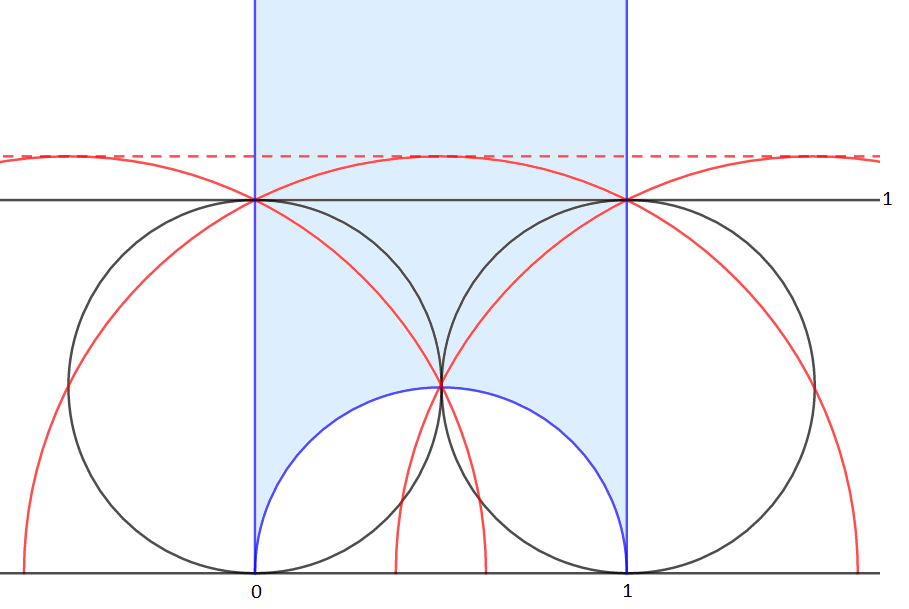
\includegraphics[width=0.5\linewidth]{pic2}
		\end{figure}\\
		\noindent 
		Рассмотрим геодезическую $m$ пересекающую треугольник в каких-то точках.\\
		\begin{figure}[h]
			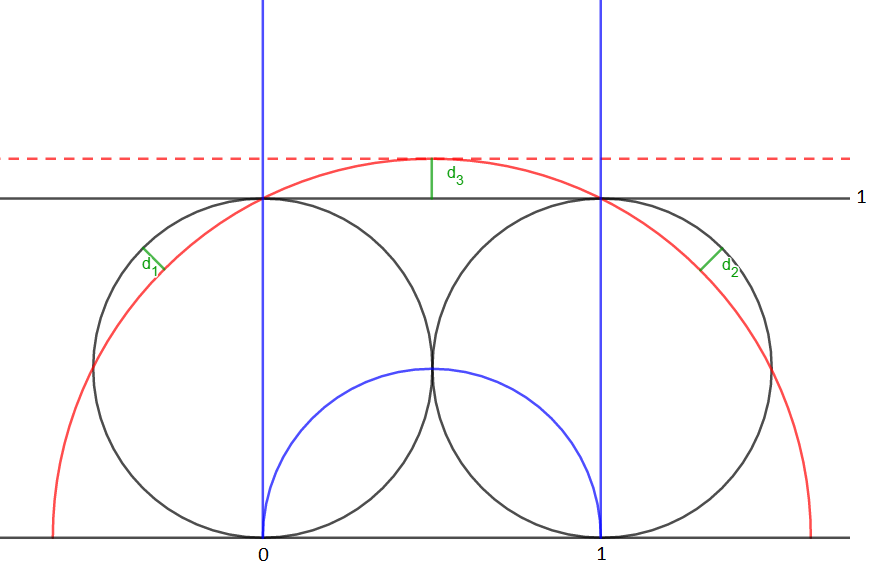
\includegraphics[width=0.5\linewidth]{pic6}
		\end{figure}
		\noindent
		Заметим что если геодезическая не пересекает какой-либо орицикл, то расстояние до нее от непересекаемого орицикла положительное, а следовательно меньше $-\ln\frac{\sqrt{5}}{2}$. Тогда если расстояние от каждого орицикла до геодезической отрицательное, то она обязана пересекать все орициклы. Тогда можно заметить, что если у геодезической нет общих точек с пунктирной линией, то расстояние $d_3$ от неё до $o(1,0)$ будет меньше $-\ln\frac{\sqrt{5}}{2}$. Если общих точек с пунктирной линией 2, то либо $d_1$, либо $d_2$ уменьшатся и, соответственно, одно из этих расстояний будет меньше $-\ln\frac{\sqrt{5}}{2}$. В случае когда $m$ имеет ровно одну общую точку с пунктирной линией но не совпадает ни с одной из средних линий либо $d_1$, либо $d_2$ уменьшится, так как $m$ будет сдвинуто в какую-то сторону относительно $l$, а при подобном параллельном переносе одна из величин $d_1,d_2$ растет, а другая уменьшается. 
		
		
		
		\newpage
		\subsubsection*{\textbf{В}}
		Рассмотрим расстояние от орицикла до вертикальной геодезической\\
		\begin{figure}[h]
			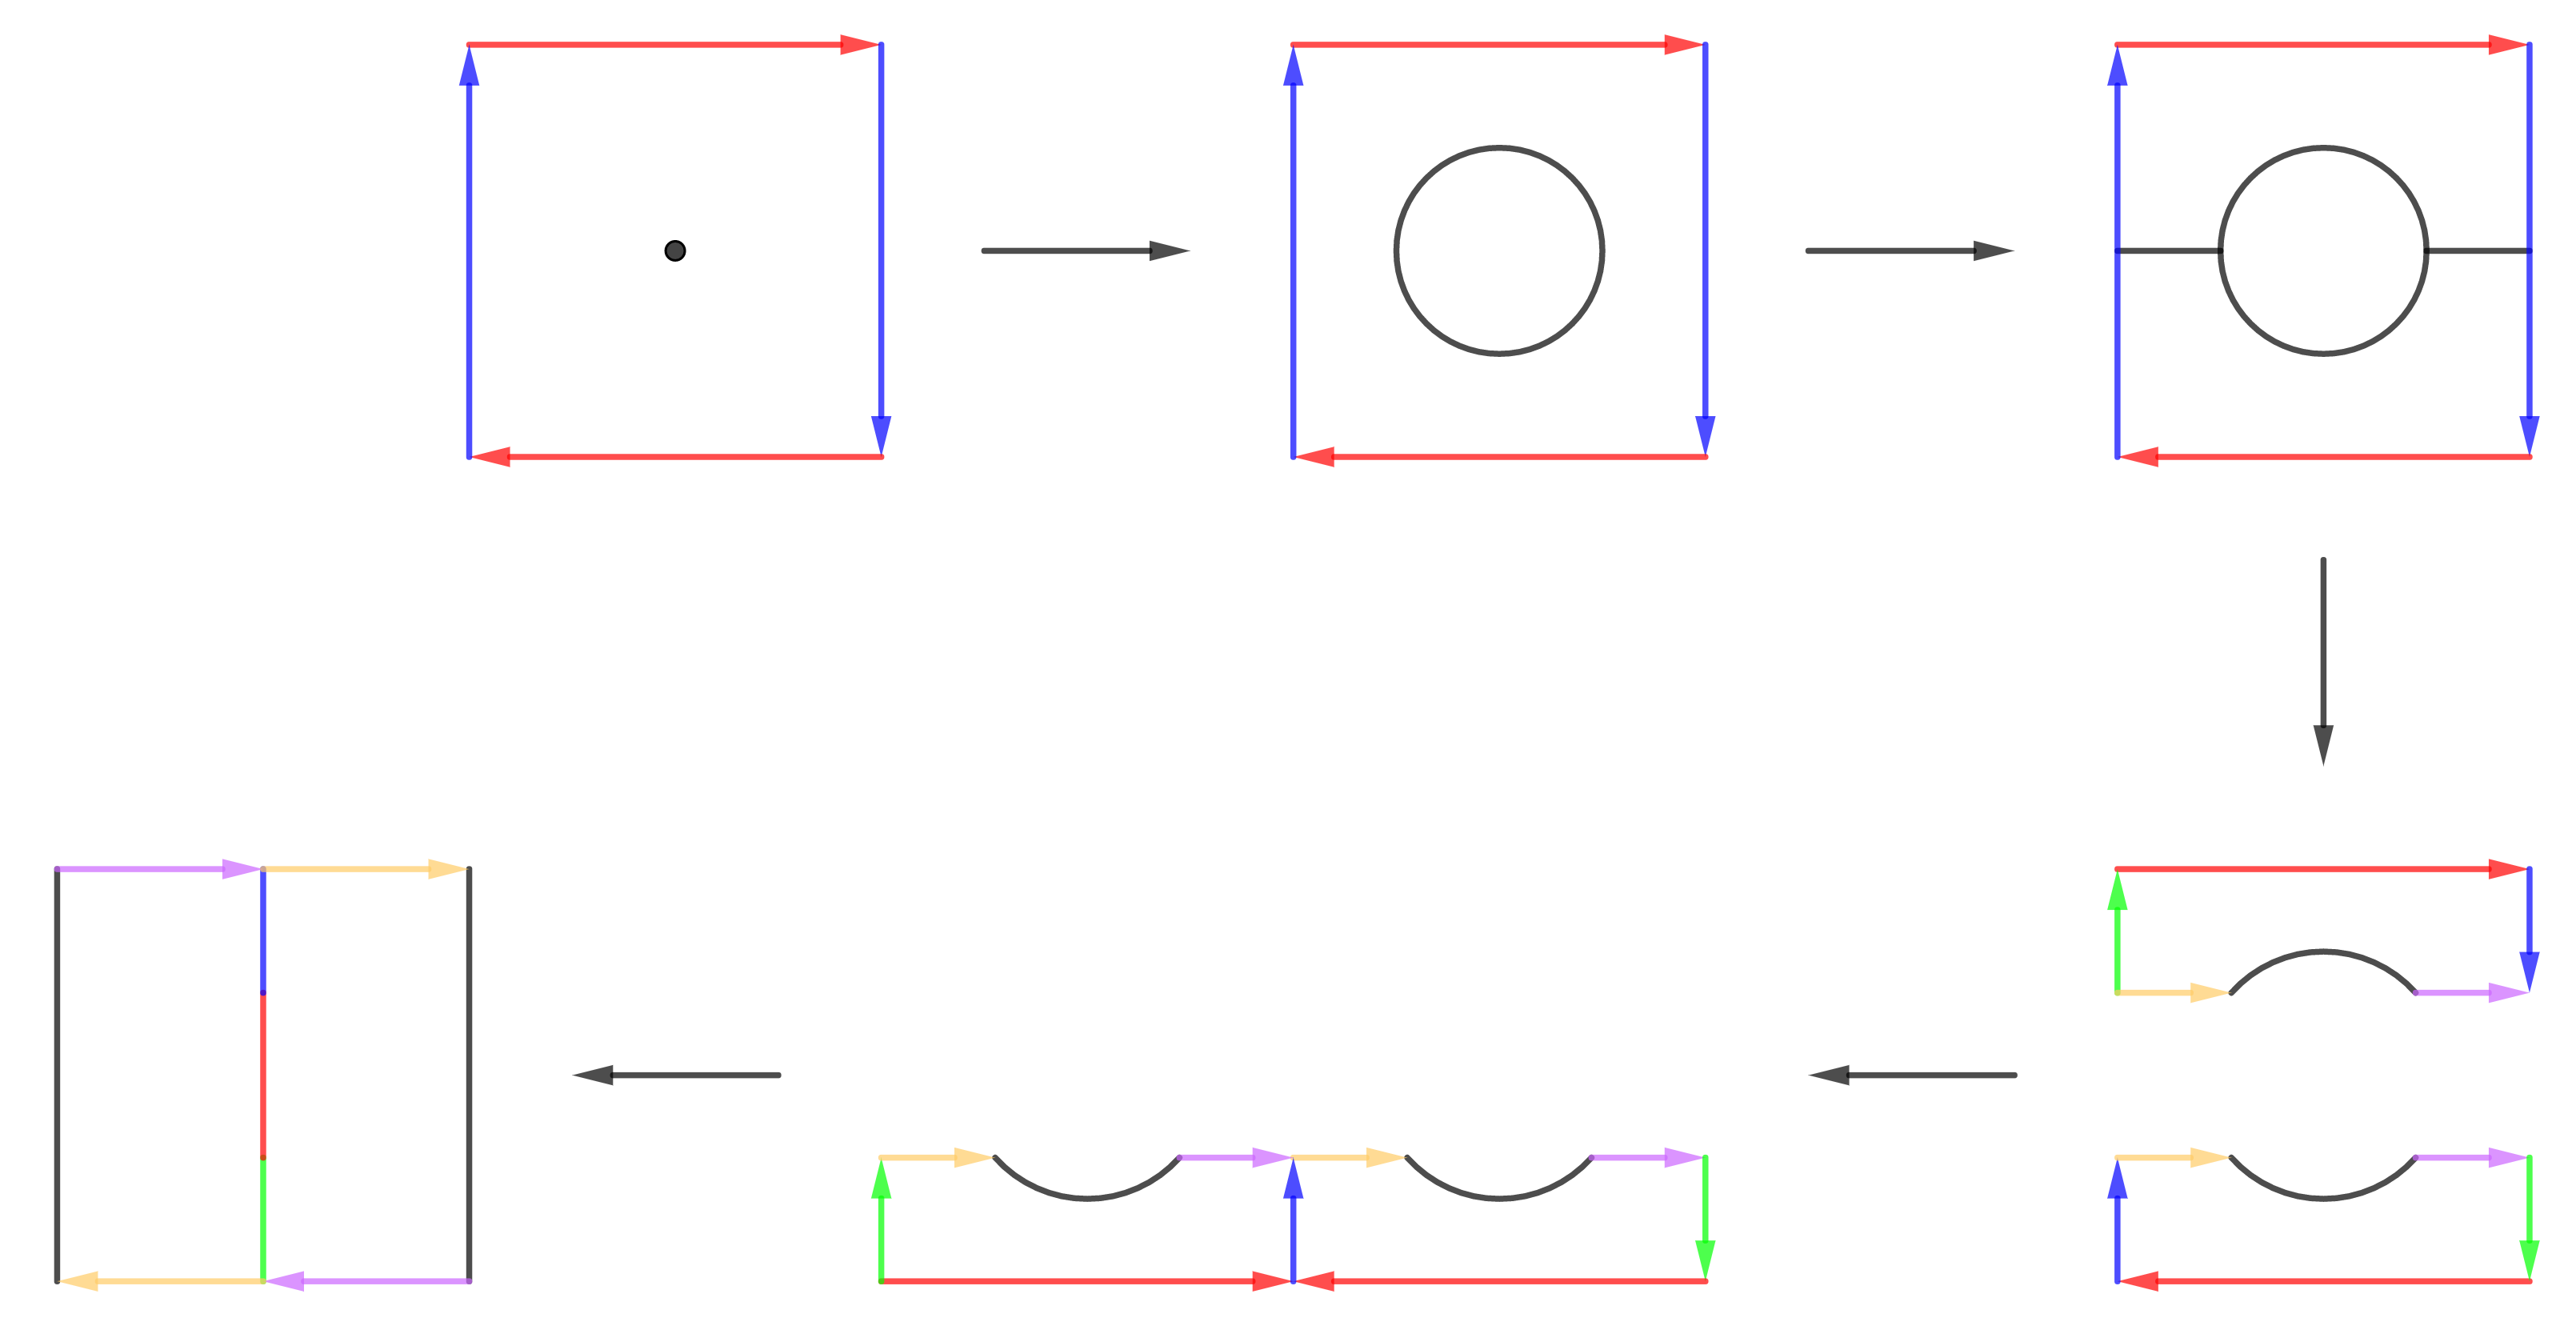
\includegraphics[width=0.5\linewidth]{pic4}
		\end{figure}\\
		\noindent
		Если орицикл это $o(p,q)$, а геодезичесая это $g$, то $d(o(p,q), g) = \ln(2q^2 |x - \frac{p}{q}|)$, это cледует из того что диаметр маленького орицикла равен $\frac{1}{q^2}$, а диаметр большого $2|x - \frac{p}{q}|$.\\
		Теперь перейдем к старой конструкции, но добавим к ней все орициклы вида $\frac{p}{q},\ \text{gcd}(p,q) = 1$, а также другие орициклы которые можно получить сдвинув полученную картинку на $n \in \mathbb{Z}$, то есть орициклы вида $\frac{p+nq}{q},\ \text{gcd}(p,q) = 1$. Так мы получим все круги Форда и круги, получаемые сдвигом кругов форда на любое целое число:\\
		\begin{figure}[h]
			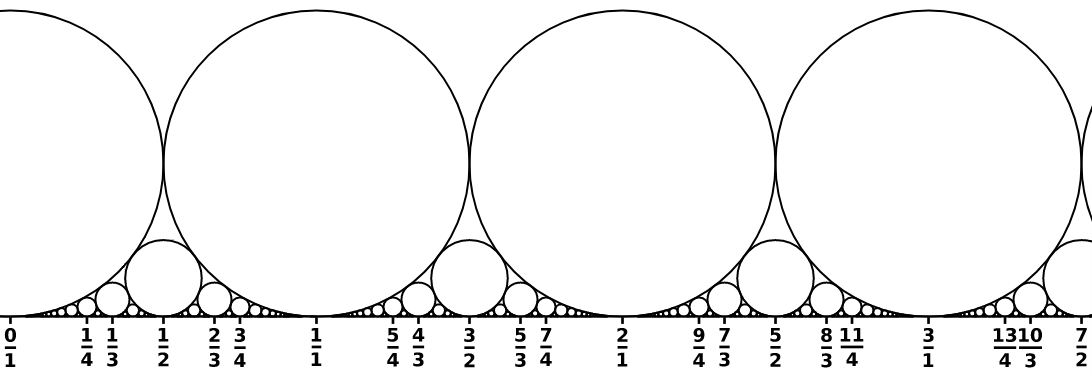
\includegraphics[width=0.5\linewidth]{pic5}
		\end{figure}\\
		\noindent 
		Добавим геодезическую $g$ в точке $a = \frac{1}{2} + \frac{\sqrt{5}}{2}$ (на рисунке отмечена зеленым)\\
		\begin{figure}[h]
			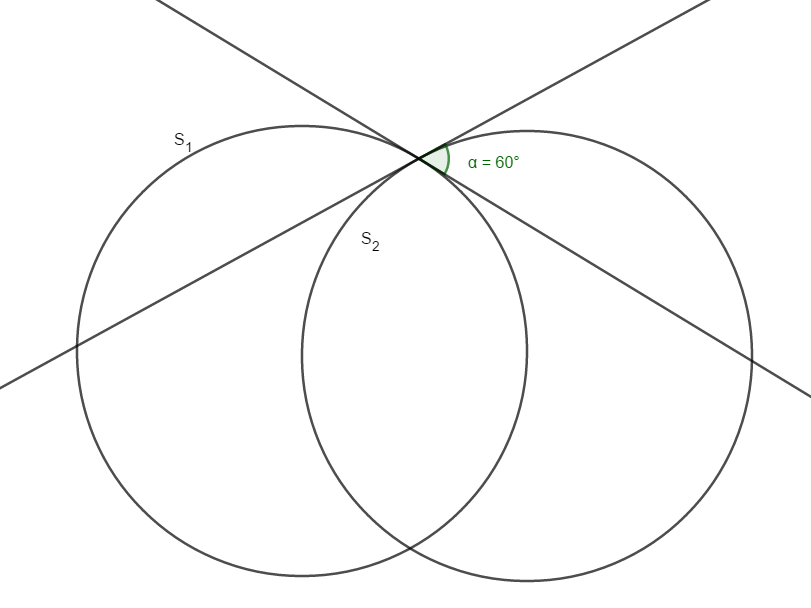
\includegraphics[width=0.5\linewidth]{pic3}
		\end{figure}\\
		\noindent 
		Так как $a$ иррационально, то геодезическая пересекает бесконенчое число кургов форда и бесконечно много треугольников с вершинами в точках касания кругов форда с абсолютой. Заметим что в каждом из таких треугольников найдется орицикл, для которого выполнено:
		\begin{gather*}
			d(o, g) < -\ln\frac{\sqrt{5}}{2}
		\end{gather*}
		Это следует из (2Б)\\
		\\
		\\
		Теперь докажем что при $x = a = \frac{1}{2} + \frac{\sqrt{5}}{2}$ и $\delta > 0$ только конечное число кругов Фордаможет удовлетворять неравенству
		\begin{gather*}
			d(o, g) < -\ln\frac{\sqrt{5}}{2} - \delta
		\end{gather*}
		Пусть $l$ геодезическая с концами $\{\frac{1}{2} - \frac{\sqrt{5}}{2}, \frac{1}{2} + \frac{\sqrt{5}}{2}\}$. Заметим что для неё $d(o,l) = -\ln\frac{\sqrt{5}}{2}$ для всех кругов Форда которые она пересекает, и $d(o,l) > -\ln\frac{\sqrt{5}}{2}$ для всех остальных.\\
		Так как геодезические $g,l$ имеют общий конец (точка $\frac{1}{2} + \frac{\sqrt{5}}{2}$), то существует точка $g_1 \in g$ такая что все круги Форда пересекающие отрезок соединяющий $g_1$ с точкой $a$, удовлетворяют неравенству
		\begin{gather*}
			|d(g,a) - d(l,a)| < \delta\\
			d(g,a) \geqslant -\ln\frac{\sqrt{5}}{2} - \delta
		\end{gather*}
		С другой стороны геодезическая $g$ без отрезка соединяющего $g_1$ с точкой $a$, пересекает только конечное число окружностей Форда, то есть только конечное число кругов Форда может удовлетворять 
		\begin{gather*}
			d(o,g) < -\ln\frac{\sqrt{5}}{2} - \delta
		\end{gather*}
		Таким образом мыдоказали теорему гурвица